\documentclass{beamer} %[12pt]
\usepackage{xcolor}
%\usetheme{boadilla}
%\usetheme{malmoe}
%\usetheme{copenhagen}
%\usecolortheme{rose}
\usecolortheme{beaver}
\usepackage{pgf, graphics}
\usepackage{graphicx}
%\usepackage[left=3cm,top=3cm,right=3cm,nohead,nofoot]{geometry}
\usepackage{hyperref}
\usepackage{setspace}
\usepackage[square]{natbib}
\usepackage{amsmath}
\usepackage{amssymb}
\usepackage{verbatim}
\usepackage{color}
\usepackage{fancyvrb}
\usepackage{bbm}

\begin{filecontents}{ref.bib}
\end{filecontents}

%\usetheme{EastLansing}
%\usepackage{natbib}
\bibliographystyle{apalike}
% make bibliography entries smaller
%\renewcommand\bibfont{\scriptsize}
% If you have more than one page of references, you want to tell beamer
% to put the continuation section label from the second slide onwards
\setbeamertemplate{frametitle continuation}[from second]
% Now get rid of all the colours
\setbeamercolor*{bibliography entry title}{fg=black}
\setbeamercolor*{bibliography entry author}{fg=black}
\setbeamercolor*{bibliography entry location}{fg=black}
\setbeamercolor*{bibliography entry note}{fg=black}
% and kill the abominable icon
\setbeamertemplate{bibliography item}{}


\newcommand{\hl}[1]{\colorbox{yellow}{#1}}
\newcommand{\hlblue}[1]{\colorbox{green}{#1}}
\newcommand{\hlblu}[1]{\colorbox{cyan}{#1}}
\newcommand{\hlred}[1]{\colorbox{cyan}{#1}}
\newcommand{\hlre}[1]{\colorbox{pink}{#1}}
\newcommand{\hlgreen}[1]{\colorbox{pink}{#1}}
\newcommand{\hlgree}[1]{\colorbox{green}{#1}}



\DeclareMathOperator*{\argmax}{\arg\!\max}

\DeclareMathOperator*{\argmin}{\arg\!\min}


\newcommand{\specialcell}[2][c]{%
  \begin{tabular}[#1]{@{}c@{}}#2\end{tabular}}



%\setbeamersize{text margin left=.5cm,text margin right=.5cm}
\newenvironment{changemargin}[2]{%
  \begin{list}{}{%
    \setlength{\topsep}{0pt}%
    \setlength{\leftmargin}{#1}%
    \setlength{\rightmargin}{#2}%
    \setlength{\listparindent}{\parindent}%
    \setlength{\itemindent}{\parindent}%
    \setlength{\parsep}{\parskip}%
  }%
  \item[]}{\end{list}}
\setbeamertemplate{navigation symbols}{}%remove navigation symbols
\usepackage{color}
\newcommand{\hilight}[1]{\colorbox{yellow}{#1}}
\setbeamertemplate{footline}[page number]

\begin{document}


\title[dedup]{Today:  1-D Categorical \\ Bar, Spine, Rose, Pie \\ Statistical Tests for Categorical Data \\ Wednesday:  2-D Categorical}


\author[Samuel L. Ventura]{\\
  \large{Sam Ventura\\36-315}}
\institute[CMU Statistics]{Department of Statistics\\Carnegie Mellon University}
\date{\today}


\begin{frame}
	\maketitle
	
\end{frame}


\begin{frame}\frametitle{Friday's Oral Evaluation Graphic}
	\small
	
	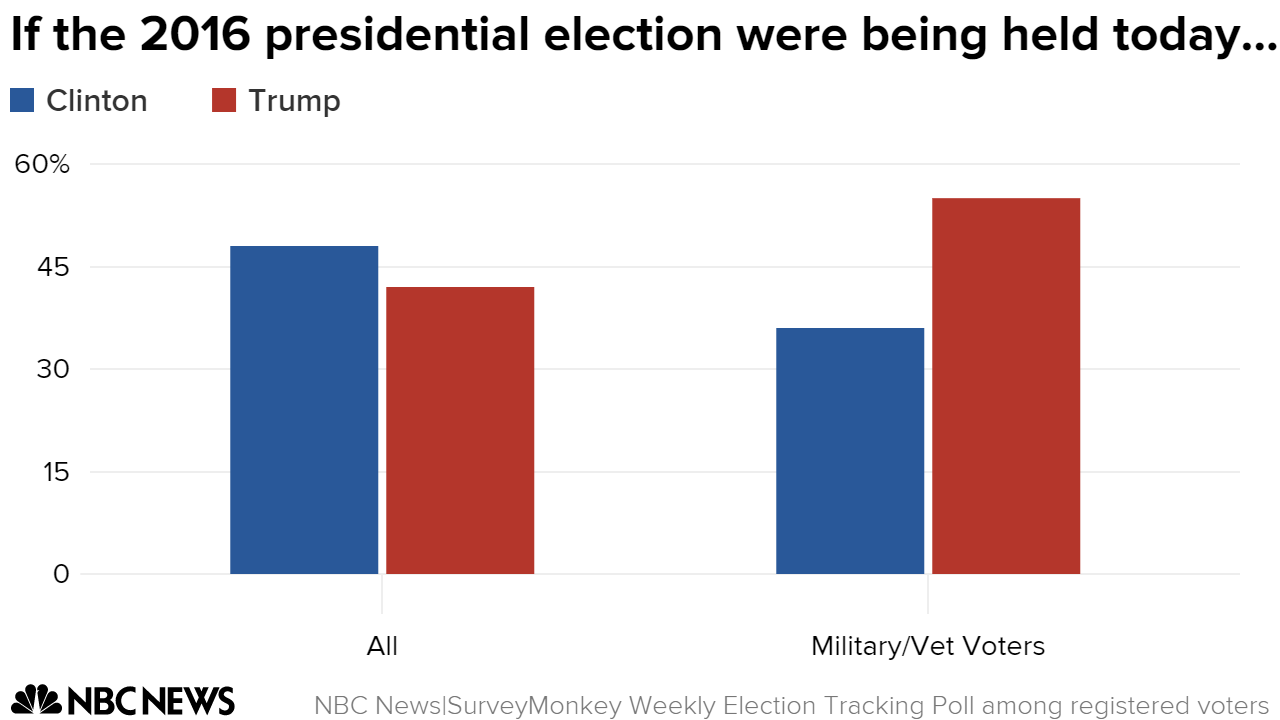
\includegraphics[width = \linewidth]{pres.png}
	
\end{frame}

\begin{frame}\frametitle{What Does a Bar Chart Show?}
	\small
	
	\textbf{Marginal Distribution}:  %Probability that the categorical variable ($X$) takes each particular categorical value ($x$)
	
	\vskip 3 cm
	
	\textbf{Empirical Distribution}:  %Our best estimate of the marginal distribution of the categorical variable we plotted, given the data we observed
	
	
	
	\vskip 10 cm
	
\end{frame}


\begin{frame}\frametitle{Bar Charts:  Counts vs. Proportions}
	\small
	
	\textbf{Counts/Frequencies of each category}:  %Give us info about sample size\\
	
	%But we could also get this by just including the sample size in the title of the chart
	
	\vskip 1 cm
	
	\textbf{Proportions}:  %Can get some additional (statistical) information:
	
	%Want to estimate $P(X = x)$ -- we'll call this $\hat{p}_X(x)$
	
	%Standard error associated with our estimate of $\hat{p}_X(x)$?
	
	%Confidence interval around our estimate of $\hat{p}_X(x)$?
	
	\vskip 10 cm
	
\end{frame}



\begin{frame}\frametitle{Chi-Square Test for Independence}
	\small
	
	\textbf{Chi-squared test}:  Statistical test used to determine whether there is a significant difference between the expected frequencies and the observed frequencies in one or more categories (of a categorical variable).
	
	\vskip 0.25 cm
	
	2-D Categorical:  Used to test differences in the conditional distributions (more on this Wednesday)
	
	\vskip 0.25 cm
	
	1-D Categorical:
	
	\vskip 10 cm
	
\end{frame}



\begin{frame}\frametitle{Computing and Interpretting the Chi-Square Test}
	\small
	
	\textbf{Test Statistic}:  
	
	\vskip 5 cm
	
	\textbf{Interpretation}:  
	
	\vskip 10 cm
	
\end{frame}


\end{document}
